\documentclass[letterpaper]{article}
\usepackage[utf8]{inputenc}
\usepackage[spanish]{babel}
\usepackage{amssymb, amsmath, mathtools}
\usepackage{graphicx}
\usepackage{lipsum}
\usepackage{dsfont}
\usepackage[margin=1.3cm,
vmargin={1.3cm,1.3cm},
includefoot]{geometry}
\usepackage{setspace}
\usepackage{subcaption}
\usepackage{tocloft}
\usepackage{upgreek}
\usepackage{amsthm}
\usepackage{graphicx}
\usepackage{paralist}
\usepackage{fancyhdr}
\usepackage{lmodern}
\usepackage{tcolorbox}
\usepackage{color}
\usepackage{tikz}
\tcbuselibrary{skins,breakable}
\pagestyle{fancy}

\renewcommand{\headrulewidth}{0pt}
\renewcommand{\footrulewidth}{0.4pt}
\cfoot{\textbf{Facultad de Ciencias, UNAM}\\ \thepage}

\newcommand{\V}{\mathds{V}}

\newcommand{\W}{\mathds{W}}

\newcommand{\F}{\mathds{F}}

\newcommand{\tq}{ \quad \cdot  \backepsilon \cdot \quad }

\newcommand{\ld}{\lim\limits_{x \to 0^{+}}}

\newcommand{\li}{\lim\limits_{x \to 0^{-}}}

\newcommand{\la}{\lim\limits_{x \to a}}

\newcommand{\R}{\mathds{R}}

\renewcommand{\*}{\cdot}

\DeclarePairedDelimiter\abs{\lvert}{\rvert}%

\newcommand{\Iden}{\begin{pmatrix}
		1 & 0 & 0\\
		0 & 1 & 0\\
		0 & 0 & 1 
\end{pmatrix}}

\newcommand{\ExiEscuela}{\textbf{Facultad de Ciencias, UNAM}}

\newtcolorbox{ejercicio}[1]{beamer,colback=white!90!white, colframe=black, title=Ejercicio #1}

\makeatletter
\renewcommand*\env@matrix[1][*\c@MaxMatrixCols c]{%
	\hskip -\arraycolsep
	\let\@ifnextchar\new@ifnextchar
	\array{#1}}
\makeatother

\newtheorem{theorem}{Teorema}[section]
\theoremstyle{definition}
\newtheorem{definition}{Definición}

\begin{document}
\begin{center}
	\textbf{\large Matemáticas para las Ciencias II}\\
	\textbf{ Semestre 2020-1}\\
	Prof. Pedro Porras Flores\\
	Ayud. Irving Hérnandez Rosas \\
	Merino Peña Kevin Ariel\\ 317031326\\
	\textbf{Proyecto I}
\end{center}
\rule{17cm}{0.3mm}

\noindent Realice los siguientes ejercicios, escribiendo el procedimiento claramente. Y recuerden que estos proyectos se entregan de manera individual en la plataforma de google classroom. 	
	% -----------------------------------------------------
	% Problema uno
	% -----------------------------------------------------
	
	  \noindent1. De la definición de parábola deduzca de manera análoga como lo hicimos en la video-clase la ecuación para una parábola cuyo foco se encuentra en el eje $x$, es decir $$y^2 = 4px.$$ 
	
	\begin{definition}
		El conjunto de los puntos del plano $ \tq $ que están a la misma distancia de una recta dada $ D $ y de un punto $ \vec{F} $, que no esté sobre $ D $, recibe el nombre de \textbf{parábola}
	\end{definition}
	Para deducir la ecuación de la parábola supongamos que la coordenadas de $ \vec{F} = (p,0) $ y que la recta D está descrita por $ w = (-p,y) \quad \forall y \in \R $, Luego por la definición que hemos tomado de prábola tenemos que 
	\begin{align*}
	||\vec{u} - \vec{F} || &= || \vec{u} - \vec{w} || && \text{Por definición de distancia} \\
	||(x,y) - (p,0) || &= || (x,y) - (-p,y) || && \text{Los valores de dichos vectores  } \\
	||(x -p,y)|| &= || (x +p,y-y)|| && \text{Restando de manera directa} \\
	\sqrt{<(x -p,y),(x -p,y)>} &= \sqrt{<(x +p,0),(x +p,0)>} && \text{Definición de la norma en vectores } \\
	\sqrt{(x -p)^2 +y^2} &= \sqrt{(x +p)^2 +(0)^2} && \text{Calculando el producto interior  } \\
	(x -p)^2 +y^2 &= (x +p)^2 +(0)^2 && \text{Factorizando } \\
	x^2 -2xp +p^2 +y^2 &= x^2 +2xp +p^2 && \text{Por distributividad  } \\
	y^2 &= 4xp && \text{Agrupando y sumando términos semejantes}
	\end{align*}
	
	\begin{figure}[h!]
		\centering
		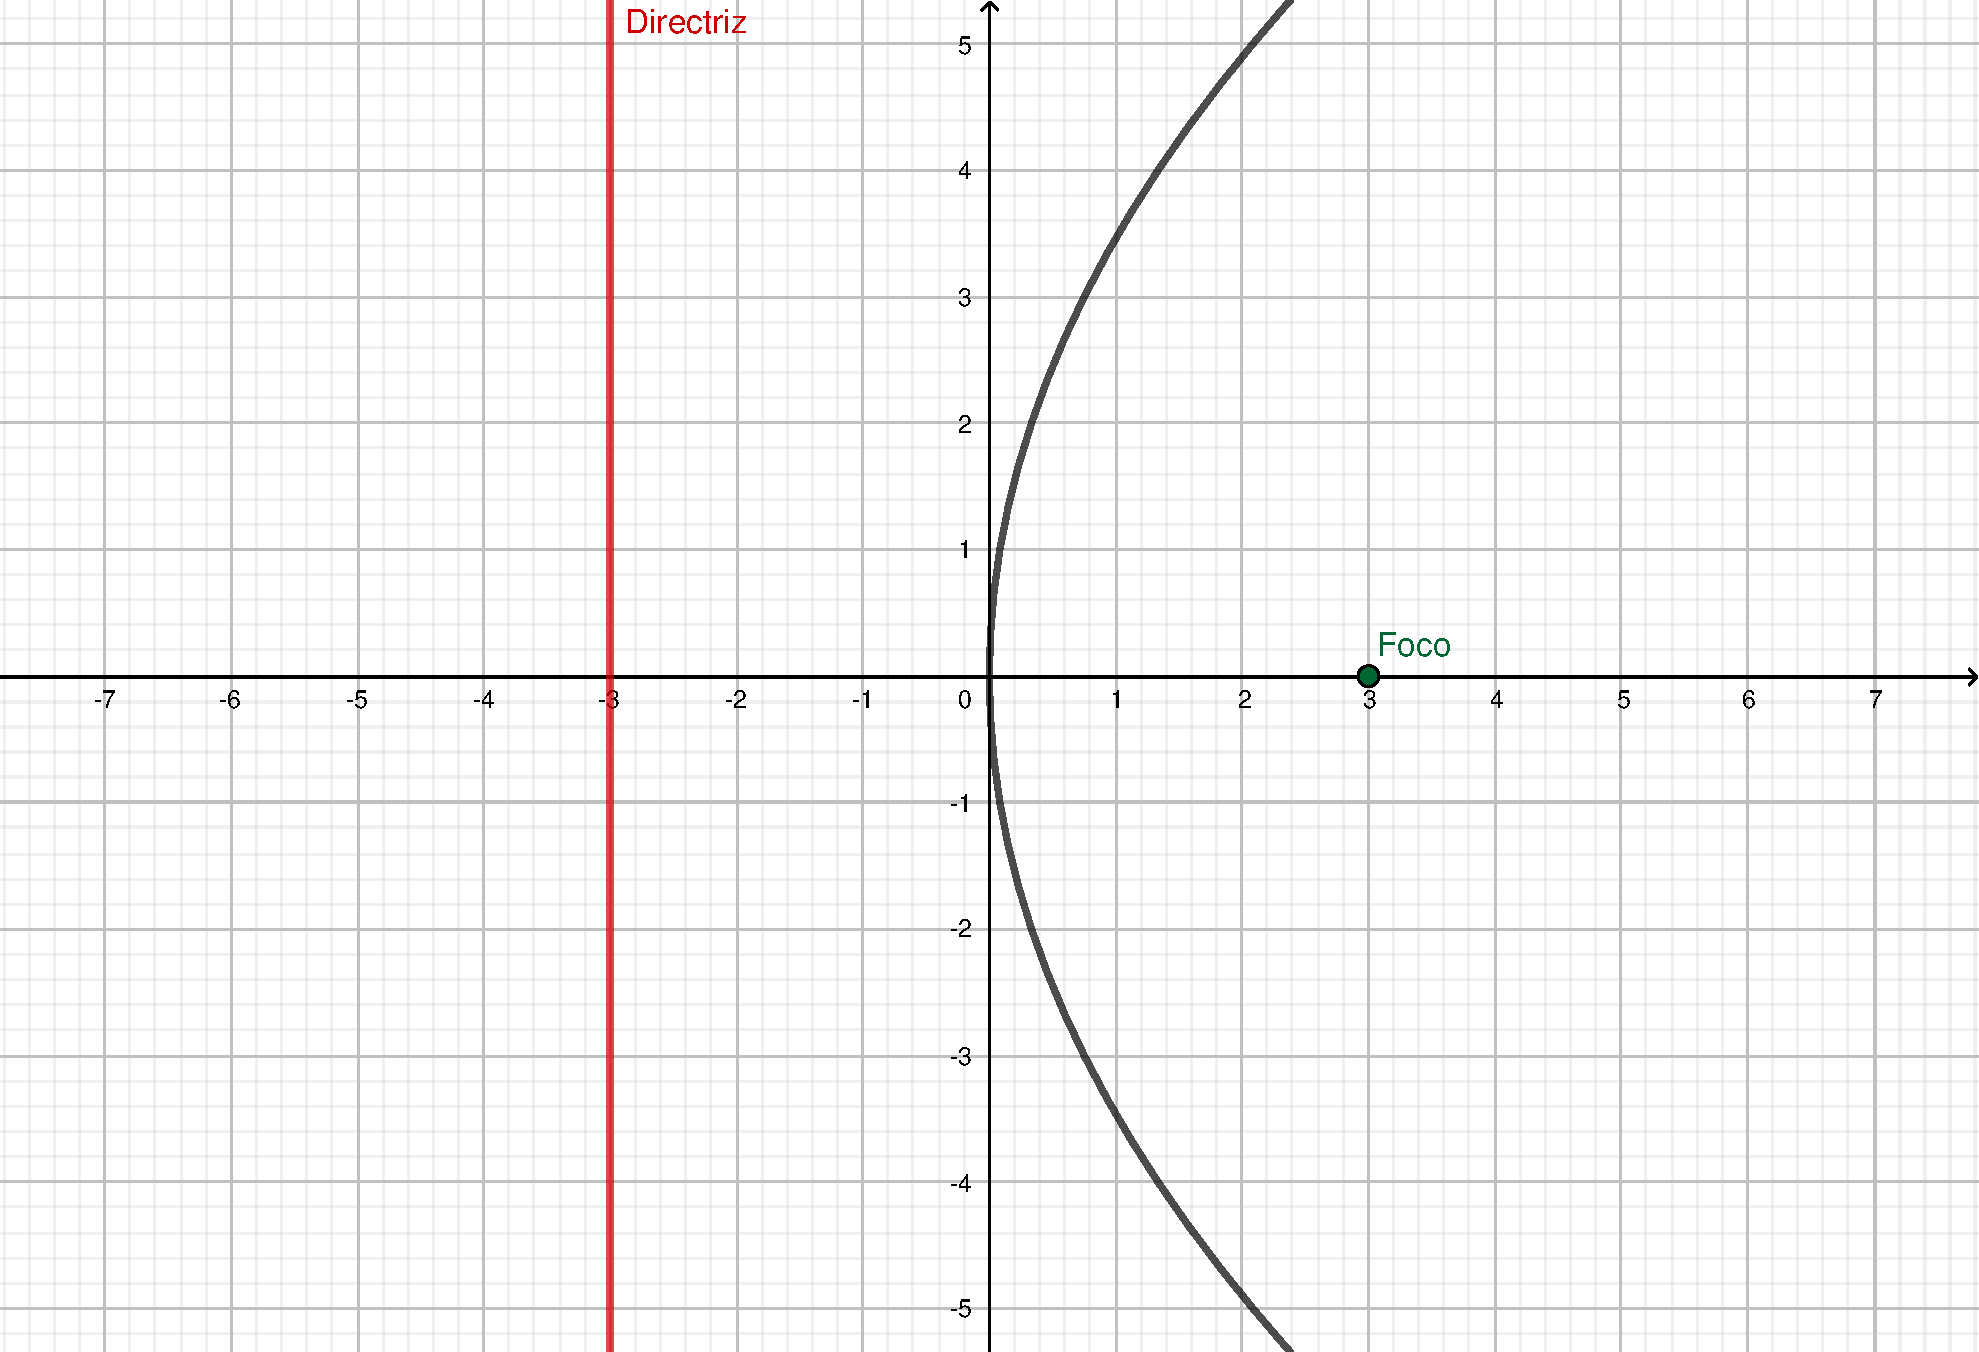
\includegraphics[width=9cm]{Parabola}
		\caption{Parábola con foco sobre el eje $x$.}
		\label{F1}
	\end{figure}
	
	% -----------------------------------------------------
	% Problema dos
	% -----------------------------------------------------
	\newpage
	\noindent2. De igual manera que se hizo en clase deduzca la ecuación de una elipse cuyos focos se encuentran sobre el eje $y$, esto es: $$\dfrac{x^2}{b^2} + \dfrac{y^2}{a^2}=1$$
	\begin{definition}
		Dados dos puntos $ \vec{F}_1, \vec{F}_2 $ del plano $ \R^2 $ tales que la suma de las diatancias de $ \vec{u} $ a $ \vec{F}_1 $ y $ \vec{F}_2 $ es una constante positiva mayor que $ d( \vec{F}_1, \vec{F}_2) $ recibe el nombre de \textbf{elipse}
		A $ \vec{F}_1, \vec{F}_2 $ se les conoce como focos y la recta que los contiene se llama eje principal
 	\end{definition}
 Ahora vamos a deducir la equación de la \textbf{elipse}.
 Hagamos las siguientes suposiciones; 
 \begin{itemize}
 	\item $ a $ es la distancia entre los vértices $ \vec{v}_1 $ y $ \vec{v}_2 $
 	\item la suma de las distancias que separan a $ \vec{u} $ de $ \vec{F}_1 $ y $ \vec{F}_2 $ es $ 2a $
 	\item $ \vec{u} = (x,y) $, $ \vec{F}_1 = (0,c) $ y $ \vec{F}_2 = ( 0,-c) $ 
 \end{itemize}
por lo que, empleando la definición de la elipse
\begin{align*}
	|| \vec{u} - \vec{F}_2 || + || \vec{u} - \vec{F}_1 || &= 2a && \text{Definición de elipse}\\
	|| (x,y) - (0,-c) || + || (x,y) - (0,c) || &= 2a && \text{Definición de los vectores}\\
	|| (x,y + c)|| + || (x,y -c)|| &= 2a && \text{Suma en vectores}\\
	 \sqrt{x^2 + (y+c)^2} + \sqrt{x^2 + (y-c)^2} &= 2a && \text{Definición de norma de un vector}\\
	 \sqrt{x^2 + (y+c)^2} &= 2a - \sqrt{x^2 + (y-c)^2}  && \text{Sumando inverso aditivo}\\
	 x^2 + (y+c)^2 &= 4a^2 -4a\sqrt{x^2 + (y-c)^2} + x^2 + (y-c)^2 && \text{Elevando al cuadrado ambos lados}\\
	 x^2 + y^2 + 2yc +c^2 &= 4a^2 -4a\sqrt{x^2 + (y-c)^2} + x^2 + y^2 -2yc +c^2 && \text{Desarrollando el cuadrado}\\
	 2yc &= 4a^2 -4a\sqrt{x^2 + (y-c)^2} -2yc && \text{Eliminando términos iguales}\\
	 4yc &= 4a^2 -4a\sqrt{x^2 + (y-c)^2} && \text{Sumando $  2yc $}\\
	 yc &= a^2 -a\sqrt{x^2 + (y-c)^2} && \text{Dividiendo entre 4}\\
	 a\sqrt{x^2 + (y-c)^2} &= a^2 - yc && \text{Despejando un término}\\
	 a^2(x^2 + (y-c)^2) &= a^4 - 2a^2yc + y^2c^2 && \text{Elevando ambos al cuadrado}\\
	 a^2(x^2 + y^2 - 2yc +c^2) &= a^4 - 2a^2yc + y^2c^2 && \text{Desarrolando los exponentes}\\
	 a^2x^2 + a^2y^2 - 2a^2yc +a^2c^2 &= a^4 - 2a^2yc + y^2c^2 && \text{Por distributividad}\\
	 a^2x^2  - y^2c^2+ a^2y^2 &= a^4 - a^2c^2 && \text{Eliminando términos iguales}\\
	 a^2x^2 + a^2y^2 - y^2c^2 &= a^4 - a^2c^2 && \text{Despejando }\\
	 a^2x^2 + y^2(a^2 - c^2) &= a^2(a^2 - c^2) && \text{Factorizando adecuadamente}\\
\end{align*}
Observemos que $ 0<c<a \implies c^2 < a^2 $ por lo que $ a^2 - c^2 > 0 $ definimos $ b^2 = a^2 - c^2 $ notemos que $ b^2 > 0, b>0 $ entonces 
\begin{align*}
	 a^2x^2 + y^2(a^2 - c^2) &= a^2(a^2 - c^2) && \text{Del resultado que obtuvimos}\\
	 a^2x^2 + y^2b^2 &= a^2b^2 && \text{Usando la observación anterior}\\
	 \dfrac{x^2}{b^2} + \dfrac{y^2}{a^2} &= 1 && \text{Dividiendo todo por $ a^2b^2 $}\\
\end{align*}
	\begin{figure}[ht!]
		\centering
		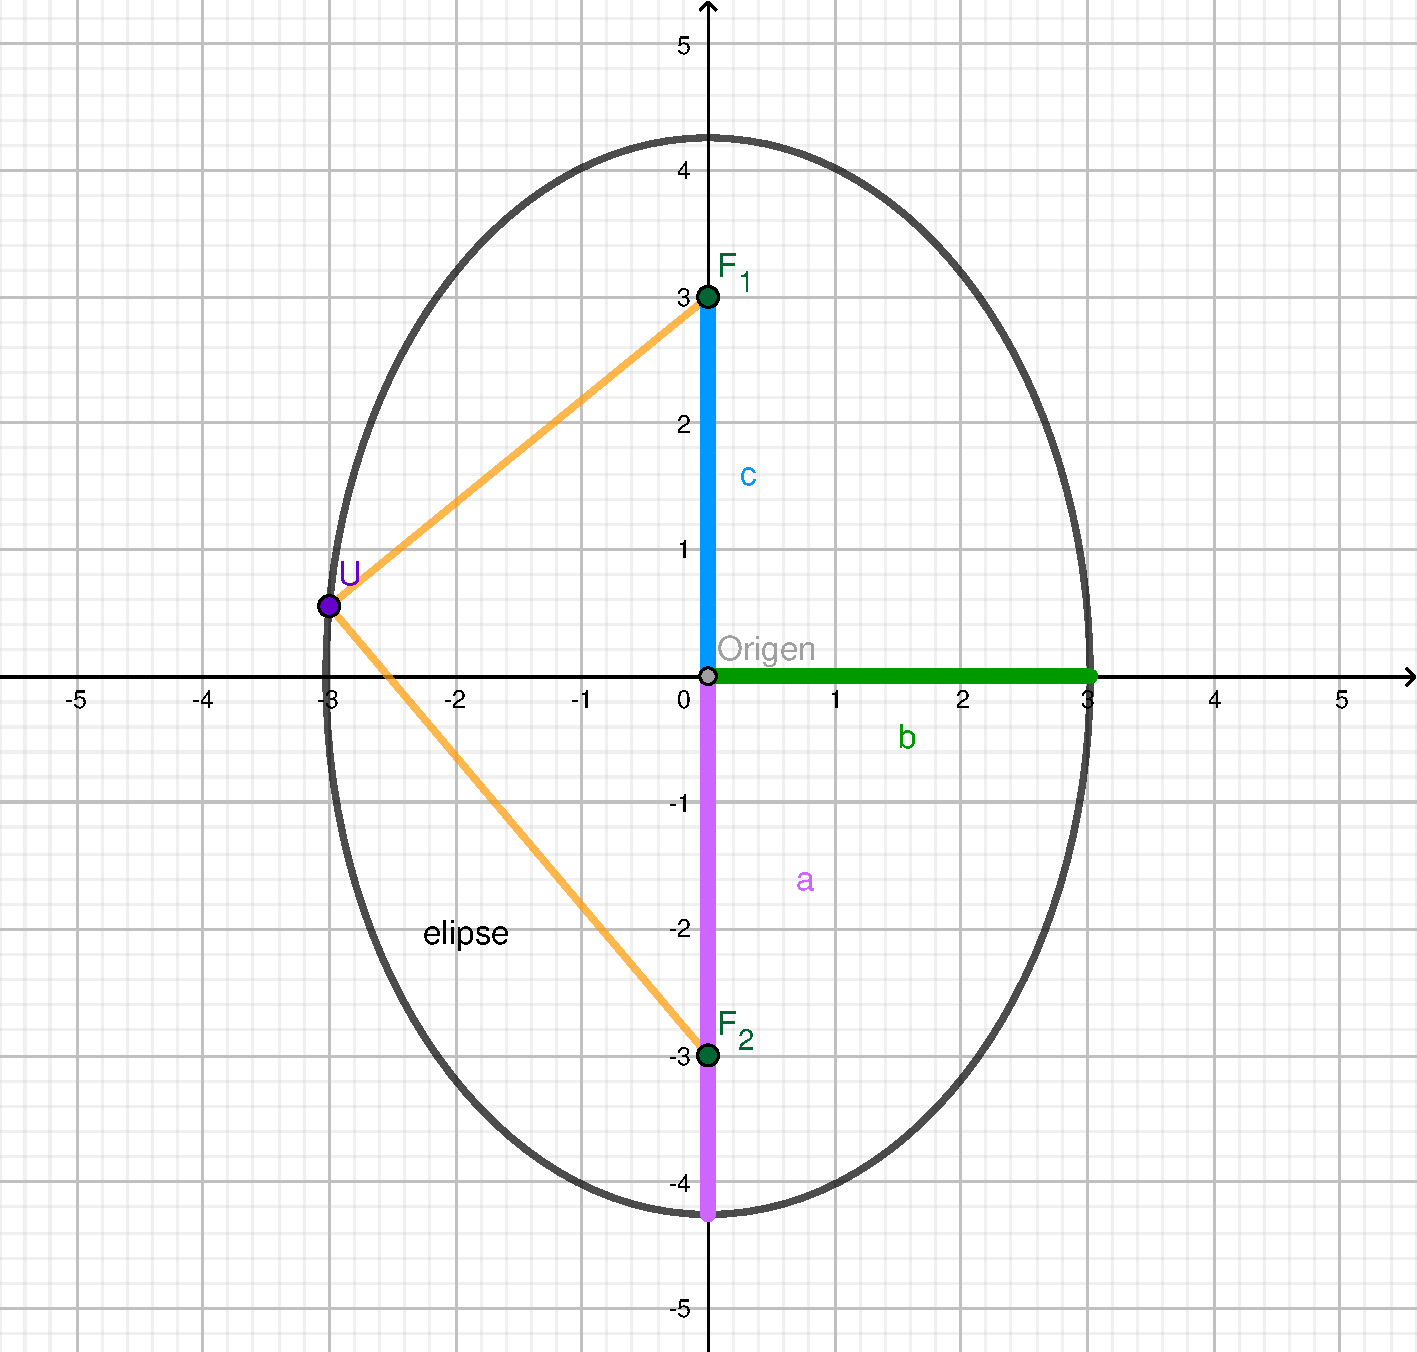
\includegraphics[width=9cm]{Elipse}
		\caption{Elipse con focos sobre el eje $y$.}
		\label{F1}
	\end{figure}
	
	% -----------------------------------------------------
	% Problema tres
	% -----------------------------------------------------
	
	\newpage
	\noindent3. Deduzca la ecuación de la hipérbola de la definición, sin importar donde estén los focos, es decir ya sea que muestre: $$\dfrac{x^2}{a^2} -  \dfrac{y^2}{b^2} = 1 \text{ o }  \dfrac{x^2}{b^2} - \dfrac{y^2}{a^2}=1$$
	\begin{definition}
		Para dos puntos datos $ \vec{F}_1 $ y $ \vec{F}_2 $ del plano $ \R^2 $, el conjunto de puntos $ \vec{u} = (x,y) $ del plano tales que el valor absoluto de la diferencia de las distancias que separan a los puntos $ \vec{F}_1 $ y $ \vec{F}_2 $ de $ \vec{u} $ es una constante menor que $ d(\vec{F}_1,\vec{F}_2) $ es una \textbf{hipérbola}
	\end{definition}
	Deduzcamos la ecuación de la hiérbola, cuyo centro es el origen con focos $ \vec{F}_1 = (c,0) $ y $ \vec{F}_2 = (-c,0) $\\ Supongamos que la distance del vértice al origen es $ a $. Además la distancia de cada punto $ \vec{u} $ a $ \vec{F}_1 $ y $ \vec{F}_2 $ es igual a $ 2a $\\Para deducir la ecuación consideremos
	\begin{align*}
	\abs{||\vec{u} - \vec{F}_1|| - || \vec{u} - \vec{F}_2||} &= 2a && \text{Por definición de hipérbola}\\ 
	||\vec{u} - \vec{F}_1|| - || \vec{u} - \vec{F}_2|| &= \pm 2a && \text{Definición de valor absoluto}\\ 
	\sqrt{ <\vec{u} - \vec{F}_1, \vec{u} - \vec{F}_1> }  - \sqrt{< \vec{u} - \vec{F}_2, \vec{u} - \vec{F}_2 >} &= \pm 2a && \text{Por definición de distancia}\\ 
	\sqrt{ <(x-c,y), (x-c,y)> }  - \sqrt{< (x+c,y),(x+c,y) >} &= \pm 2a && \text{Así elegimos los vectores}\\ 
	\sqrt{ (x-c)^2 +y^2 }  - \sqrt{ (x+c)^2 + y^2} &= \pm 2a && \text{Aplicando producto interno}\\ 
	\sqrt{ (x-c)^2 + y^2 }  &= \pm 2a + \sqrt{ (x+c)^2 + y^2} && \text{Despejando}\\
	(x-c)^2 + y^2 &= 4a^2 \pm 4a\sqrt{ (x+c)^2 + y^2} + (x+c)^2 + y^2 && \text{Elevando al cuadrado}\\ 
	(x-c)^2  &= 4a^2 \pm 4a\sqrt{ (x+c)^2 + y^2} + (x+c)^2 && \text{Eliminando t. iguales}\\ 
	x^2 -2xc +c^2  &= 4a^2 \pm 4a\sqrt{ (x+c)^2 + y^2} + x^2+2xc+c^2 && \text{Desarrolando}\\ 
	-2xc &= 4a^2 \pm 4a\sqrt{ (x+c)^2 + y^2} +2xc && \text{Eliminando iguales}\\ 
	-4xc &= 4a^2 \pm 4a\sqrt{ (x+c)^2 + y^2} && \text{Despejando términos}\\ 
	-xc &= a^2 \pm a\sqrt{ (x+c)^2 + y^2} && \text{Dividiendo entre 4}\\ 
	\end{align*}
	\begin{align*}
	-(xc + a^2)&= \pm a\sqrt{ (x+c)^2 + y^2} && \text{Despejando términos}\\ 
	a^4 + 2a^2cx + x^2c^2 &=  a^2((x+c)^2 + y^2) && \text{Elevando al cuadrado}\\ 
	a^4 + 2a^2cx + x^2c^2 &=  a^2(x^2 + 2xc +c^2 + y^2) && \text{Desarrollando cuadrados}\\ 
	a^4 + 2a^2cx + x^2c^2 &=  a^2x^2 + 2a^2xc +a^2c^2 + a^2y^2 && \text{Distribuyendo }\\ 
	(c^2 - a^2)x^2 &=  a^2(c^2-a^2) + a^2y^2 && \text{Despejando }\\
	b^2x^2 &=  a^2b^2 + a^2y^2 && \text{Despejando }\\
	b^2x^2 - a^2y^2 &=  a^2b^2 && \text{Restando  $ a^2y^2 $ }\\
	\dfrac{x^2}{a^2} - \dfrac{y^2}{b^2} &=  1 && \text{Dividiendo por $  a^2b^2 $ }\\
	\end{align*}
	\begin{figure}[ht!]
		\centering
		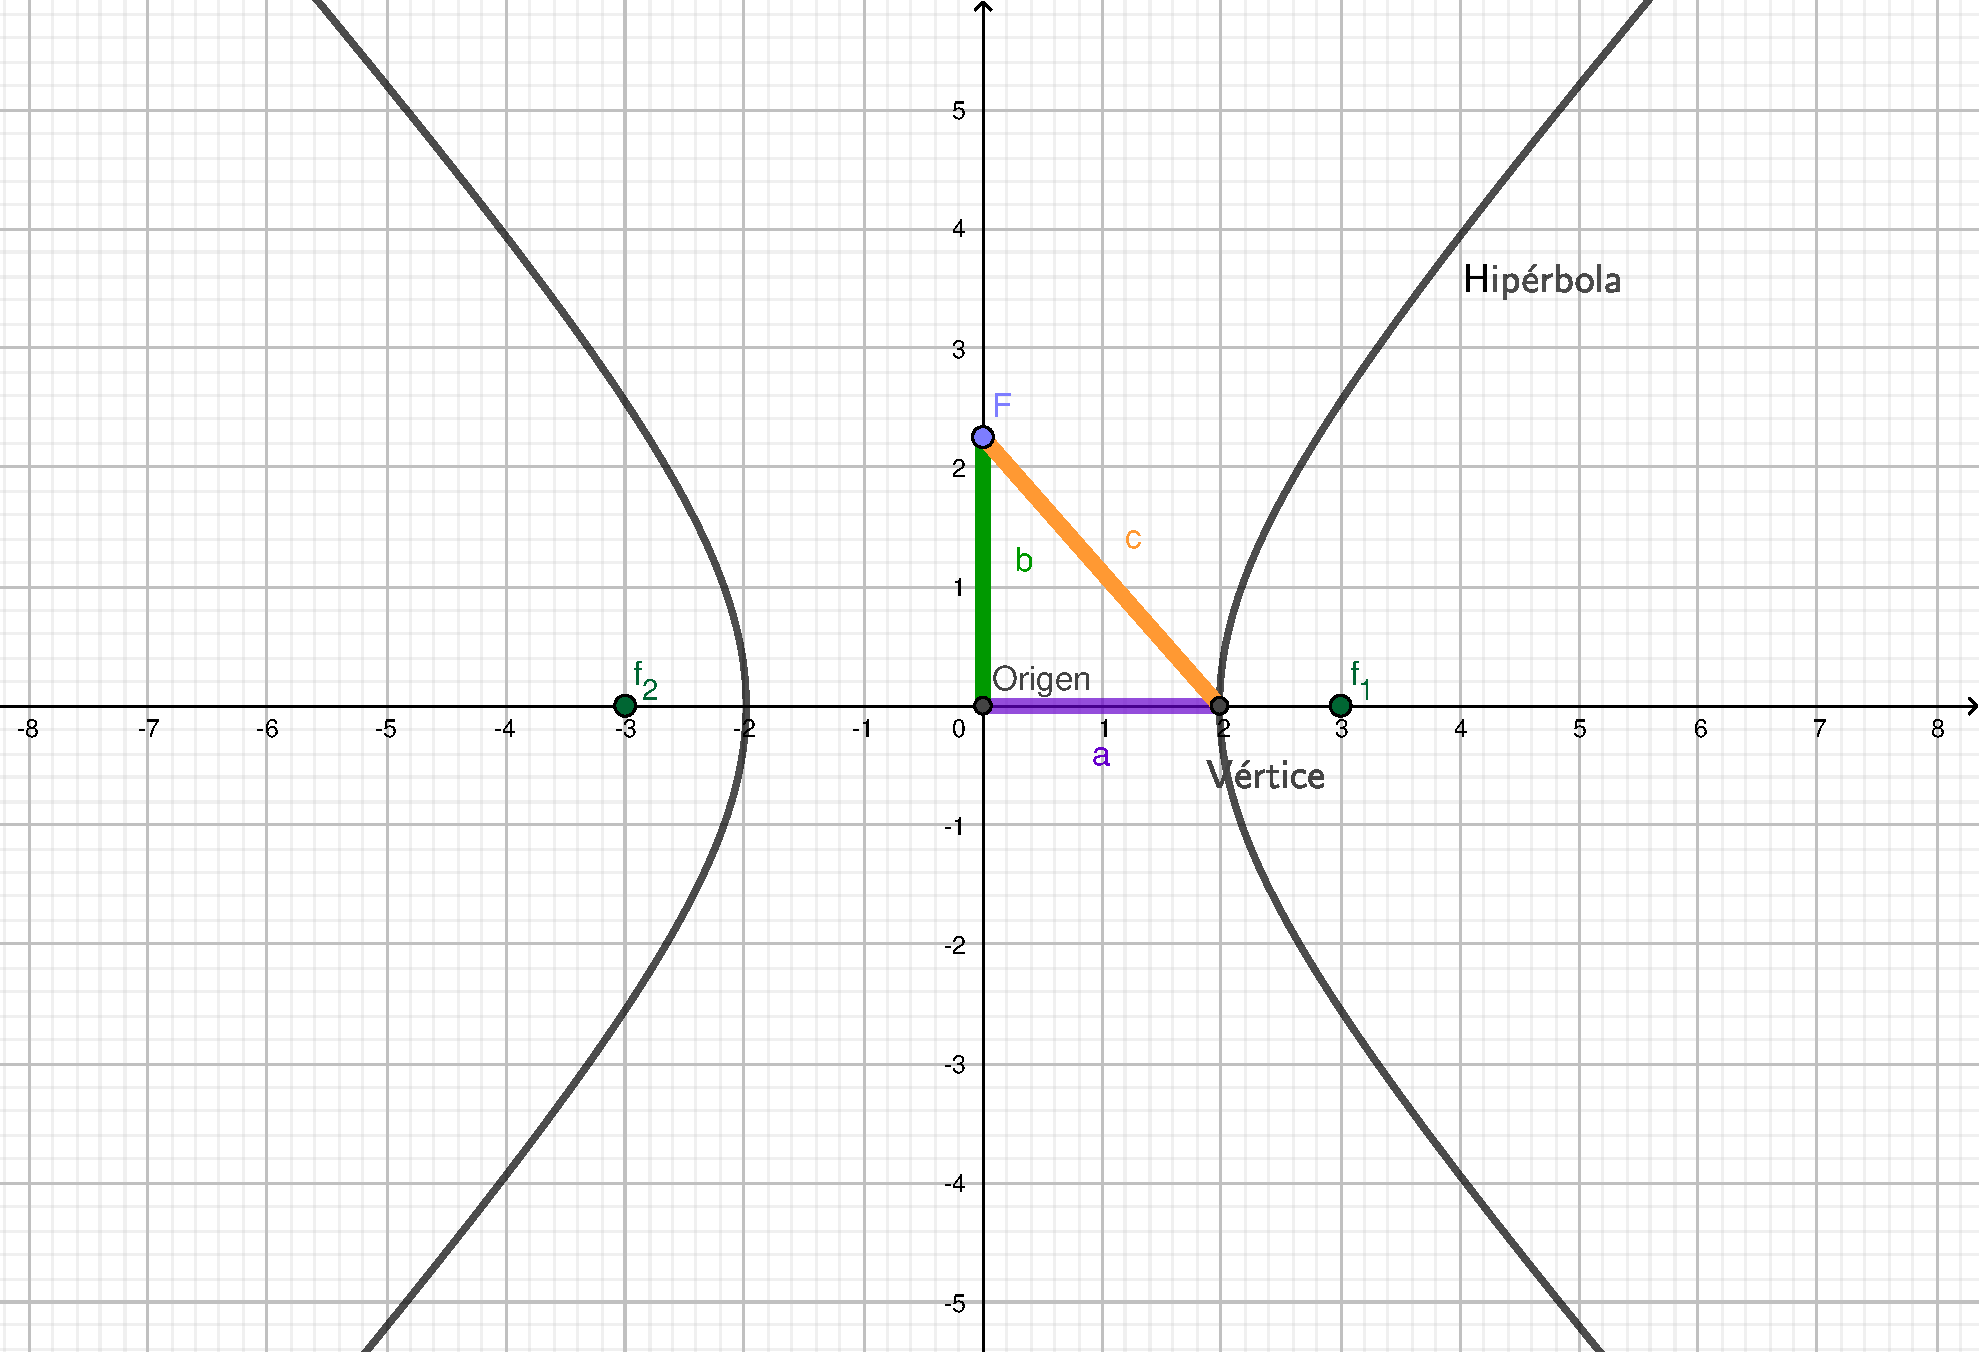
\includegraphics[width=7cm]{Hiperbola}
		\caption{Hipérbola con focos sobre el eje $x$.}
		\label{F1}
	\end{figure}
	
	
	

\end{document}